\documentclass[conference]{IEEEtran}

\usepackage{amsmath,amssymb,amsfonts}
\usepackage{graphicx}
\usepackage{booktabs}
\usepackage{multirow}
\usepackage{array}
\usepackage{cite}
\usepackage{url}
\usepackage{microtype}
\usepackage{makecell}

% Slight vertical adjustment for IEEE PDF margin compliance
\addtolength{\topmargin}{0.03in}
\addtolength{\textheight}{-0.03in}

\begin{document}
%
% paper title
% Titles are generally capitalized except for words such as a, an, and, as,
% at, but, by, for, in, nor, of, on, or, the, to and up, which are usually
% not capitalized unless they are the first or last word of the title.
% Linebreaks \\ can be used within to get better formatting as desired.
% Do not put math or special symbols in the title.
\title{Radiometry-Aware Evaluation of Cross-Sensor Satellite
Image Super-Resolution}


% author names and affiliations
% use a multiple column layout for up to three different
% affiliations
\author{\IEEEauthorblockN{Mohammad Alnakhli}
\IEEEauthorblockA{\textit{Department of Electrical Engineering} \\
\textit{Prince Sattam Bin Abdulaziz University}\\
Wadi Addwasir 11991, Saudi Arabia \\
M.alnakhli@psau.edu.sa}
\and

\IEEEauthorblockN{Fatimah Emad Eldin}
\textit{Department of Statistical Research}\\
\IEEEauthorblockA{Cairo University}
 Cairo 12613, Egypt \\
12422024441586@pg.cu.edu.eg
\and
\IEEEauthorblockN{Ahad Majed Alsulami}
\IEEEauthorblockA{ \textit{Software and AI Department} \\ \textit{SARsatX},\\ Jeddah 23326 , Saudi Arabia\\Email: ahad.alsulami@sarsatx.com}
\and
\IEEEauthorblockN{Mohsn Alawi Alsaidi–
}
\IEEEauthorblockA{\textit{Department of Aerospace Engineering}\\ \textit{ King Fahd University of Petroleum and Minerals} \\Dhahran 31261, Saudi Arabia\\ 
Email: s202066080@kfupm.edu.sa}
\and
\IEEEauthorblockN{Layan Mohammed Alharbi}
\IEEEauthorblockA{ \textit{
Department of Computer Science and Artificial Intelligence}\\ \textit{Umm Al-Qura University}\\
Makkah, Saudi Arabia\\ 
Email:S444001325@uqu.edu.sa}
}

 




% use for special paper notices
%\IEEEspecialpapernotice{(Invited Paper)}




% make the title area
\maketitle

% As a general rule, do not put math, special symbols or citations
% in the abstract
\begin{abstract}
Real cross-sensor satellite image super-resolution (SR) differs from
synthetic SR because the source and target observations vary not only
in spatial resolution but also in sensor-dependent radiometry.
Consequently, improvements over conventional bicubic interpolation may
reflect radiometric adaptation rather than genuine spatial-detail
recovery. This paper investigates this distinction using FLAIR-HUB
pairs from Sentinel-2, SPOT, and $0.20$~m aerial imagery at resolution
ratios of $6.4\times$, $8\times$, and $51.2\times$. Representative
convolutional, residual, attention, transformer, and diffusion-based SR
models are evaluated against both raw and symmetrically radiometrically
matched bicubic controls. Results show that apparent PSNR gains of up
to $15.01$~dB against raw bicubic interpolation become close to zero
after radiometric matching, demonstrating that a substantial fraction
of the conventional gain originates from cross-sensor radiometric
differences. Nevertheless, the SR models recover measurable spatial
information, reaching up to $5.55\times$ the sharpness of bicubic
interpolation and recovering approximately $13$--$22\%$ of target
gradient magnitude across structured land-cover classes. Incorporating
target-resolution normalized digital surface model (nDSM) information
in a focused SPOT-to-aerial case study moves the mean EDSR matched-PSNR
difference from $-0.18$~dB to $+0.02$~dB, i.e., approximate parity
with the matched control, while increasing sharpness from $3.08\times$
to $3.75\times$, improving LPIPS, and improving detail recovery in
seven of eight evaluated classes with approximately $1\%$ additional
parameters. These results indicate that real
cross-sensor SR should be evaluated jointly through radiometrically
matched fidelity, spatial-detail recovery, and perceptual quality
rather than raw PSNR alone.
\end{abstract}
 
 \begin{IEEEkeywords}
Cross-sensor super-resolution, remote sensing, satellite imagery,
radiometric matching, spatial-detail recovery, elevation guidance,
FLAIR-HUB.
\end{IEEEkeywords}
% no keywords




% For peer review papers, you can put extra information on the cover
% page as needed:
% \ifCLASSOPTIONpeerreview
% \begin{center} \bfseries EDICS Category: 3-BBND \end{center}
% \fi
%
% For peerreview papers, this IEEEtran command inserts a page break and
% creates the second title. It will be ignored for other modes.
\IEEEpeerreviewmaketitle

 \section{Introduction}
\label{sec:introduction}

High-resolution Earth observation (EO) imagery is important for
land-cover mapping, urban monitoring, agriculture, and environmental
assessment. However, satellite sensors involve inherent trade-offs
among spatial resolution, spectral resolution, revisit frequency, and
coverage. Image super-resolution (SR) provides a computational approach
for enhancing spatial information from lower-resolution observations.
Deep SR has progressed from convolutional and residual architectures
such as SRCNN and EDSR \cite{dong2016srcnn,lim2017edsr} to
attention- and transformer-based models such as RCAN and SwinIR
\cite{zhang2018rcan,liang2021swinir}, while recent remote-sensing
studies increasingly explore diffusion and prior-guided reconstruction
\cite{sgdm2025,li2025dlmsr}.

A major challenge arises when SR is applied to images acquired by
different sensors. Unlike synthetic SR, where the low-resolution image
is generated directly from the high-resolution target, real
cross-sensor observations can differ in spatial sampling, spectral
response, radiometry, illumination, acquisition time, and geometric
alignment. Recent datasets and cross-platform studies have therefore
shifted attention toward real satellite--aerial SR
\cite{aybar2024sen2naip,wang2026crossplatform}. Under such conditions,
an improvement in conventional fidelity metrics may reflect adaptation
to the target sensor's radiometry rather than genuine recovery of
missing spatial information.

Building on recent evaluation and radiometric-consistency work
\cite{aybar2024benchmark,aybar2026sen2sr}, we investigate a
complementary question: \emph{how much of the apparent improvement
of cross-sensor SR originates from radiometric adaptation, and how
much corresponds to measurable spatial-detail recovery?}

To answer it, we compare SR predictions against both raw bicubic
interpolation and a symmetrically radiometrically matched bicubic
control. Pixel fidelity is further complemented by perceptual
similarity and gradient-based spatial-detail measurements. Experiments
are conducted on FLAIR-HUB \cite{garioud2026flairhub} using three real
cross-sensor configurations: Sentinel-2$\rightarrow$SPOT
($6.4\times$), SPOT$\rightarrow$aerial ($8\times$), and
Sentinel-2$\rightarrow$aerial ($51.2\times$). Representative
convolutional, residual, attention, transformer, and diffusion-based
models are evaluated under geographically disjoint training and test
regions.

The main contributions of this work are threefold. First, we conduct
a real cross-sensor SR study spanning Sentinel-2, SPOT, and aerial
imagery, with resolution gaps from $6.4\times$ to $51.2\times$ under
geographically disjoint evaluation. Second, we introduce a
radiometrically controlled evaluation that separates apparent SR gains
from radiometric adaptation and jointly considers matched fidelity,
perceptual similarity, and spatial-detail recovery, including
land-cover-specific analysis. Third, in a focused SPOT$\rightarrow$aerial case
study, we investigate an elevation-guided SR refinement using
target-resolution normalized digital surface model (nDSM) data, which improves detail recovery in seven of
eight evaluated land-cover classes while adding approximately $1\%$
to the EDSR parameter count. The contribution is primarily an
evaluation methodology; the SR backbones are established
architectures, and no new general-purpose SR network is proposed.

\section{Related Work}
\label{sec:related}

Real-world remote-sensing SR has moved from synthetically degraded
pairs toward real cross-sensor observations. SEN2NAIP pairs
Sentinel-2 with aerial NAIP imagery \cite{aybar2024sen2naip}, and
cross-platform diffusion SR enhances satellite imagery with aerial
targets \cite{wang2026crossplatform}. OpenSR-test evaluates SR through
consistency, synthesis, and correctness rather than full-reference
fidelity alone \cite{aybar2024benchmark}, and SEN2SR enforces
radiometric and spatial consistency with the Sentinel-2 input
\cite{aybar2026sen2sr}. Table~\ref{tab:related} summarizes how the
present study complements these works: rather than proposing a new
benchmark or SR network, it measures how much of a reported
cross-sensor gain survives an explicit, symmetrically applied
radiometric control, and relates the remainder to spatial-detail,
land-cover, and elevation-guided analyses.

\begin{table}[!t]
\centering
\caption{Positioning Against Recent Real-World Remote-Sensing SR Work}
\label{tab:related}
\footnotesize
\setlength{\tabcolsep}{2.4pt}
\resizebox{\columnwidth}{!}{%
\begin{tabular}{lccccc}
\toprule
Work & \makecell{Real\\cross-sensor} & \makecell{Matched\\radiom.\ control}
& \makecell{Spatial-\\detail metric} & \makecell{Land-cover\\analysis}
& nDSM \\
\midrule
SEN2NAIP \cite{aybar2024sen2naip} & \checkmark & -- & -- & -- & -- \\
OpenSR-test \cite{aybar2024benchmark} & \checkmark & -- & \checkmark & -- & -- \\
SEN2SR \cite{aybar2026sen2sr} & \checkmark & -- & -- & -- & -- \\
Cross-platform \cite{wang2026crossplatform} & \checkmark & -- & -- & -- & -- \\
This paper & \checkmark & \checkmark & \checkmark & \checkmark & \checkmark \\
\bottomrule
\end{tabular}}
\end{table}

\begin{figure*}[!t]
    \centering
    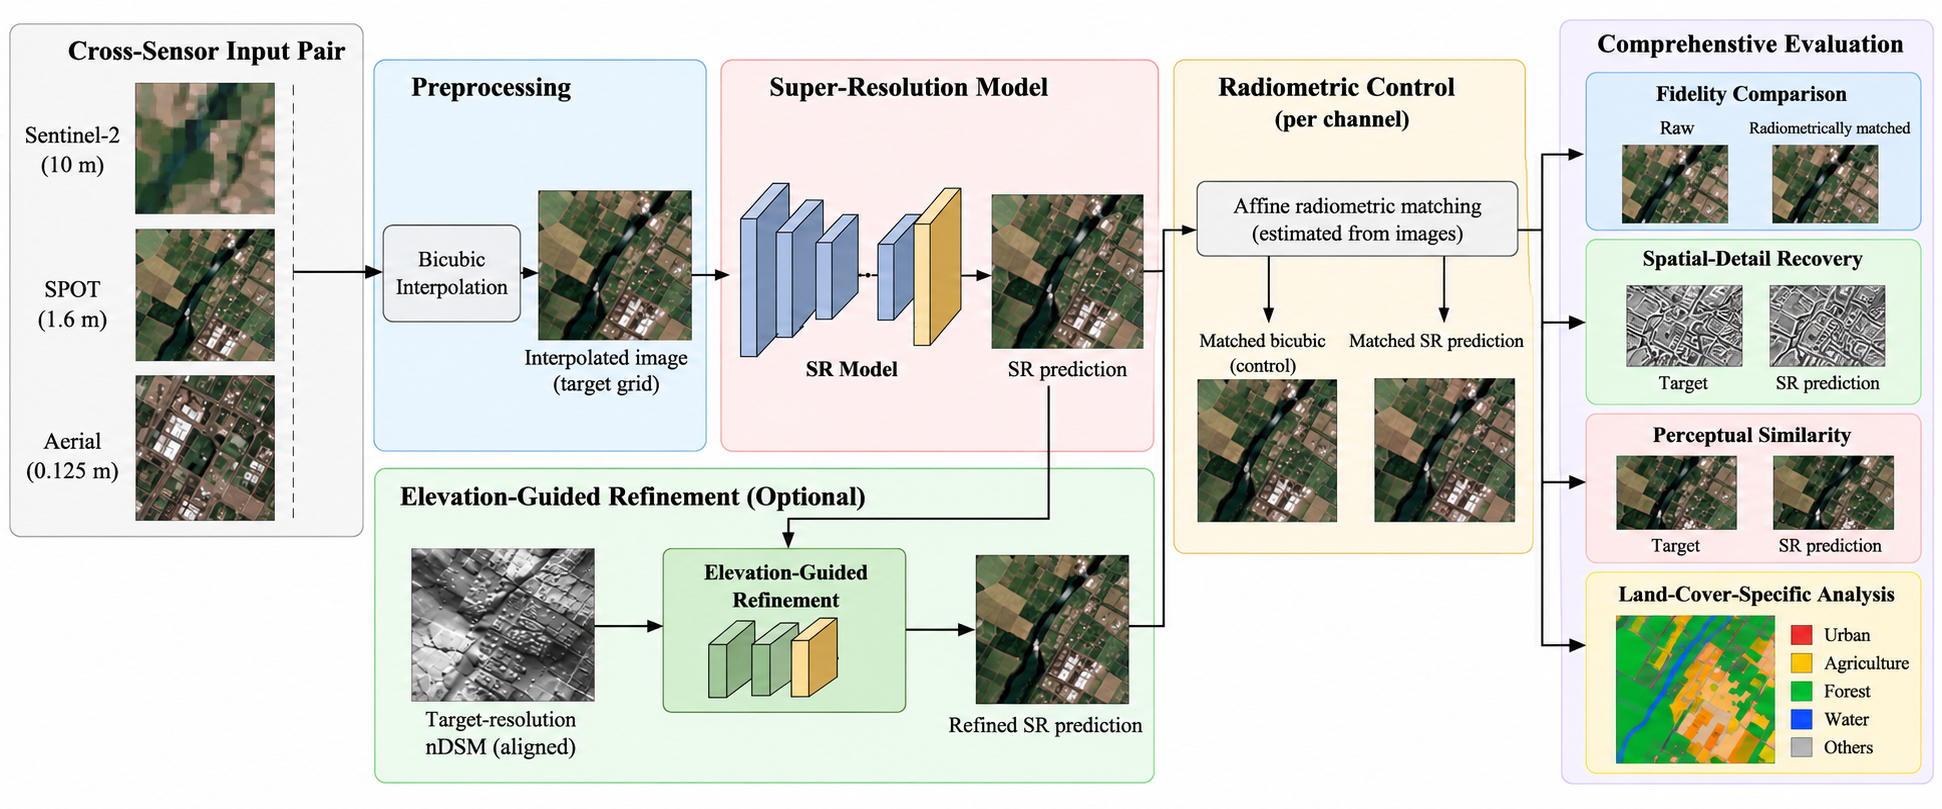
\includegraphics[width=\textwidth]{fig_framework}
    \caption{Overview of the proposed cross-sensor SR framework.
    The low-resolution observation is reconstructed by an SR model and
    evaluated using raw and radiometrically matched controls to separate
    apparent radiometric gains from spatial-detail recovery. Perceptual
    and gradient-based measures provide complementary evaluation, while
    target-resolution nDSM information can be incorporated through a
    lightweight elevation-guided refinement module.}
    \label{fig:framework}
\end{figure*}
%%%%%%%%%%%%%%%%%%%%%
\section{Proposed Radiometry-Aware Cross-Sensor SR Framework}
\label{sec:method}

The framework is summarized in Fig.~\ref{fig:framework}.



Let $\mathbf{x}\in\mathbb{R}^{H\times W\times C}$ denote a
low-resolution source-sensor observation and
$\mathbf{y}\in\mathbb{R}^{sH\times sW\times C}$ the corresponding
high-resolution target-sensor image, where $s$ is the cross-sensor
resolution ratio. The source image is first interpolated to the target
grid,
\begin{equation}
\mathbf{x}_{\mathrm{bic}}=\mathcal{U}_{s}(\mathbf{x}),
\label{eq:bicubic}
\end{equation}
where $\mathcal{U}_{s}(\cdot)$ denotes bicubic interpolation. The
regression models predict a correction to this interpolated input,

\begin{equation}
\hat{\mathbf{y}}
=
\mathbf{x}_{\mathrm{bic}}
+
f_{\theta}(\mathbf{x}),
\label{eq:sr_prediction}
\end{equation}

where $f_{\theta}(\cdot)$ is the trainable SR model and
$\hat{\mathbf{y}}$ is the reconstructed target-resolution image.
SRCNN, RCAN, and SwinIR apply $f_{\theta}$ to $\mathbf{x}_{\mathrm{bic}}$,
whereas EDSR applies it to $\mathbf{x}$ and upsamples internally; the
conditional DDPM instead samples $\hat{\mathbf{y}}$ conditioned on the
source observation.

A direct comparison between $\hat{\mathbf{y}}$ and $\mathbf{y}$ mixes
spatial reconstruction with differences in sensor radiometry.
Therefore, in addition to the raw bicubic control, a radiometrically
matched control is computed. For any image
$\mathbf{z}\in\{\mathbf{x}_{\mathrm{bic}},\hat{\mathbf{y}}\}$ and
channel $c$, a least-squares gain and offset onto the target are
estimated independently for every test image,

\begin{equation}
(\alpha_c(\mathbf{z}),\beta_c(\mathbf{z}))
=
\arg\min_{\alpha,\beta}
\left\|
\alpha \mathbf{z}_{c}
+\beta-\mathbf{y}_{c}
\right\|_2^2 ,
\label{eq:affine}
\end{equation}

and the matched image is
$\mathcal{M}(\mathbf{z})_c=\mathrm{clip}_{[0,1]}
(\alpha_c(\mathbf{z})\mathbf{z}_c+\beta_c(\mathbf{z}))$.
The bicubic control and the SR prediction each receive their own
optimal fit, $\tilde{\mathbf{x}}_{\mathrm{bic}}=
\mathcal{M}(\mathbf{x}_{\mathrm{bic}})$ and
$\tilde{\mathbf{y}}=\mathcal{M}(\hat{\mathbf{y}})$.
The control is therefore symmetric: both outputs are given the same
oracle radiometric correction, so the SR model receives no fitting
advantage that the bicubic control lacks. Ignoring clipping, the
matched squared error of channel $c$ equals
$\sigma_{y_c}^2(1-\rho_c^2)$, where $\rho_c$ is the Pearson
correlation between $\mathbf{z}_c$ and $\mathbf{y}_c$; matched PSNR
is thus invariant to any per-channel gain and offset of either output
and compares only how well its spatial structure correlates with the
target. Because the fit uses $\mathbf{y}$, the matched control is an
\emph{oracle evaluation control}: it is computed only at evaluation
time and is never available to, or used by, any model during training
or inference. It is not an operational preprocessing step. The same
procedure and code are applied identically to every model and all
three sensor configurations.

The affine model is chosen deliberately. A per-channel gain and offset
is the first-order description of inter-sensor differences in
calibration, atmospheric conditions, and illumination; it has a
closed-form solution; and, being a global per-channel mapping, it
cannot add spatial structure. Hence, an advantage remaining after
matching cannot be explained by a global linear radiometric
difference. The model also has limitations. Spectral-response
mismatch, nonlinear radiometric relations, spatially varying
illumination and shadows, and acquisition-time differences are not
captured by a per-image affine map, so part of the cross-sensor
discrepancy can remain after matching.
$\Delta_{\mathrm{matched}}$ should therefore be read as a
first-order radiometric control rather than a complete removal of
sensor effects. Two complementary PSNR differences are reported:
\begin{equation}
\Delta_{\mathrm{raw}}
=
\mathrm{PSNR}(\hat{\mathbf{y}},\mathbf{y})
-
\mathrm{PSNR}(\mathbf{x}_{\mathrm{bic}},\mathbf{y}),
\label{eq:delta_raw}
\end{equation}
and
\begin{equation}
\Delta_{\mathrm{matched}}
=
\mathrm{PSNR}(\tilde{\mathbf{y}},\mathbf{y})
-
\mathrm{PSNR}(\tilde{\mathbf{x}}_{\mathrm{bic}},\mathbf{y}).
\label{eq:delta_matched}
\end{equation}

Here, $\Delta_{\mathrm{raw}}$ measures the apparent improvement over
the conventional interpolation baseline, whereas
$\Delta_{\mathrm{matched}}$ measures the remaining fidelity difference
after symmetric radiometric correction. The gap between them is used
as an empirical diagnostic of how strongly the apparent gain depends on
radiometric differences that a global affine map can absorb. It is not
an exact decomposition of the SR gain into ``radiometric'' and
``spatial'' components, because PSNR is not additive and the two
effects interact.

Because matched PSNR alone does not quantify the amount of recovered
high-frequency information, spatial detail is evaluated using image
gradients. For an image $\mathbf{z}$ containing $N$ pixels, the mean
gradient magnitude is defined as

\begin{equation}
G(\mathbf{z})
=
\frac{1}{2}\left(
\overline{|\partial_x \mathbf{z}|}
+
\overline{|\partial_y \mathbf{z}|}
\right),
\label{eq:gradient}
\end{equation}

where $\partial_x,\partial_y$ are forward finite differences and the
bar denotes the mean over all pixels and channels. The
target-normalized spatial-detail recovery is

\begin{equation}
R_{\mathrm{detail}}(\mathbf{z})
=
\frac{G(\mathbf{z})}
     {G(\mathbf{y})},
\label{eq:detail_recovery}
\end{equation}

and \emph{sharpness} relative to interpolation is

\begin{equation}
S
=
\frac{\overline{R}_{\mathrm{detail}}(\hat{\mathbf{y}})}
     {\overline{R}_{\mathrm{detail}}(\mathbf{x}_{\mathrm{bic}})}
\approx
\frac{G(\hat{\mathbf{y}})}
     {G(\mathbf{x}_{\mathrm{bic}})},
\label{eq:bic_recovery}
\end{equation}

where $\overline{R}_{\mathrm{detail}}$ is averaged over the test set.
The first quantity indicates the fraction of target gradient magnitude
represented by the reconstruction, whereas $S$ quantifies the
increase in high-frequency content relative to bicubic interpolation
($S=1$ for bicubic itself).
Throughout the paper, \emph{gradient magnitude} refers to the absolute
quantity $G(\cdot)$, and \emph{sharpness} refers to the dimensionless
ratio $S$; the two are not used interchangeably.
Sharpness is a proxy for recovered spatial detail because bicubic
interpolation cannot create frequencies above the source Nyquist
limit, so additional gradient energy must come from the model. It
measures the \emph{amount} of high-frequency content, not its
\emph{correctness}: ringing, noise, and hallucinated texture also
increase $G$. It is therefore interpreted only together with matched
fidelity, LPIPS, and the qualitative examples.
Gradient magnitude is insensitive to additive intensity offsets but
scales with multiplicative radiometric gain; therefore, it is
interpreted jointly with the radiometrically matched fidelity analysis
rather than as a radiometrically invariant metric.

To determine whether recovery depends on scene content, the same
measure is computed over pixels belonging to land-cover class $k$,

\begin{equation}
R_{k}
=
\frac{G_{k}(\hat{\mathbf{y}})}
     {G_{k}(\mathbf{y})},
\label{eq:class_recovery}
\end{equation}

where $G_k(\cdot)$ denotes the mean gradient magnitude restricted to
class $k$, computed as the $\ell_2$ norm of central differences of
the channel-mean image and pooled over all class-$k$ pixels of the
evaluated tiles. Reporting $G_k(\mathbf{y})$ together with $R_k$ is important
because a high recovery percentage may correspond to only a small
amount of absolute detail when the target class itself contains little
high-frequency structure.

Finally, target-resolution elevation information is incorporated as an
auxiliary geometric prior. Let $\mathbf{h}$ denote the normalized nDSM
aligned with the target image. A lightweight refinement network
$g_{\phi}(\cdot)$ predicts a residual correction from the concatenated
SR output and elevation map,

\begin{equation}
\hat{\mathbf{y}}_{\mathrm{EG}}
=
\hat{\mathbf{y}}
+
g_{\phi}
\left(
[\hat{\mathbf{y}},\mathbf{h}]
\right),
\label{eq:elevation_guided}
\end{equation}

where $[\cdot,\cdot]$ denotes channel-wise concatenation. The final
convolution of $g_{\phi}$ is initialized to zero so that, at
initialization, the guided model reduces to its unguided backbone;
backbone and refinement are then trained jointly. The refinement
module contains only $11{,}299$ trainable parameters, corresponding to
approximately $1\%$ of the EDSR parameter count.

\emph{Data.} All pairs come from FLAIR-HUB \cite{garioud2026flairhub}.
Each tile covers $102.4\times102.4$~m and is co-registered across
Sentinel-2 ($10\times10$~px, 10.24~m), SPOT ($64\times64$~px,
1.6~m), and aerial imagery ($512\times512$~px, 0.20~m); the aerial
target is used at its native resolution without downsampling. All
experiments use the three RGB channels: Sentinel-2 B4/B3/B2 as the
median of 12 cloud-filtered temporal bins, the first three SPOT bands,
and the aerial RGB image. Satellite reflectance is scaled by
$1/0.3$ and aerial digital numbers by $1/255$, both clipped to
$[0,1]$. Training uses 4{,}662 tiles from seven domains (D004, D006,
D011, D017, D022, D033, D037) and testing uses 1{,}332 tiles from two
geographically disjoint domains (D040, D044). Every model is trained on
the same tiles, and every (architecture, configuration, seed) is
trained separately from scratch; no model is transferred between
sensor pairs. No separate validation split is used, and the final
epoch is evaluated without checkpoint selection.

\emph{Training.} SRCNN \cite{dong2016srcnn} (188k parameters), EDSR
\cite{lim2017edsr} (927k), RCAN \cite{zhang2018rcan} (1.01M), and
SwinIR \cite{liang2021swinir} (241k) are trained with an $\ell_1$
loss; the conditional DDPM (264k) uses the noise-prediction MSE loss
with $T{=}200$ linear-schedule steps and 200-step ancestral sampling.
All models use AdamW with a constant learning rate of
$2\times10^{-4}$, effective batch size 32 (gradient accumulation for
512-px targets), mixed precision, horizontal-flip augmentation, and
25 epochs. Hyperparameters are deliberately identical across
architectures rather than individually tuned. RCAN and DDPM are
evaluated on Sentinel-2$\rightarrow$SPOT only. The nDSM refinement
(Eq.~\ref{eq:elevation_guided}) is trained jointly with its backbone
from scratch using the same settings, with the nDSM converted to
meters, divided by 30, and clipped to $[0,1]$.

\emph{Evaluation and uncertainty.} PSNR is computed on $[0,1]$ data
over all channels per tile and averaged over the 1{,}332 test tiles.
LPIPS \cite{zhang2018lpips} uses the AlexNet variant on RGB inputs
scaled to $[-1,1]$; lower is better, and the \emph{LPIPS improvement}
plotted in Fig.~\ref{fig:perceptual} is the absolute difference
$\mathrm{LPIPS}(\mathbf{x}_{\mathrm{bic}},\mathbf{y})-
\mathrm{LPIPS}(\hat{\mathbf{y}},\mathbf{y})$, so positive values
favor the SR model. Where five seeds (7, 41, 913, 1337, 2026) are
available, values are seed means and $\pm$ denotes the sample standard
deviation across seeds of each run's test-set mean; it is neither a
per-image spread nor a confidence interval. Cells marked $\dagger$ in
Table~\ref{tab:abs} are single runs (seed 1337) and carry no
uncertainty estimate. Experiments were run on cloud GPUs via Modal.

\begin{table}[!t]
\centering
\caption{Absolute Test-Set Metrics. PSNR in dB; $S$ Is Sharpness
Relative to Bicubic (Eq.~\ref{eq:bic_recovery}); S2 Denotes Sentinel-2}
\label{tab:abs}
\footnotesize
\setlength{\tabcolsep}{3pt}
\resizebox{\columnwidth}{!}{%
\begin{tabular}{llcccc}
\toprule
Config. & Model & \makecell{PSNR\\raw} & \makecell{PSNR\\matched}
& LPIPS$\downarrow$ & $S$ \\
\midrule
\multirow{6}{*}{\makecell[l]{S2$\rightarrow$\\SPOT\\($6.4\times$)}}
 & Bicubic & 14.25 & 35.24 & 0.562 & 1.00 \\
 & SRCNN & 28.94 & 34.62 & 0.334 & 0.59 \\
 & EDSR & 29.26 & 34.93 & 0.318 & 1.00 \\
 & RCAN & 29.16 & 34.77 & 0.329 & 0.65 \\
 & SwinIR$^{\ast}$ & 24.63 & 34.58 & 0.381 & 0.91 \\
 & DDPM$^{\dagger}$ & 26.00 & 33.59 & 0.288 & 3.58 \\
\midrule
\multirow{4}{*}{\makecell[l]{SPOT$\rightarrow$\\aerial\\($8\times$)}}
 & Bicubic & 10.63 & 21.74 & 0.913 & 1.00 \\
 & SRCNN & 17.68 & 21.56 & 0.851 & 1.90 \\
 & EDSR & 17.92 & 21.57 & 0.868 & 3.22 \\
 & SwinIR$^{\dagger}$ & 17.62 & 21.40 & 0.839 & 5.55 \\
\midrule
\multirow{4}{*}{\makecell[l]{S2$\rightarrow$\\aerial\\($51.2\times$)}}
 & Bicubic & 16.44 & 21.58 & 0.871 & 1.00 \\
 & SRCNN$^{\dagger}$ & 17.53 & 20.99 & 0.849 & 1.43 \\
 & EDSR$^{\dagger}$ & 17.80 & 21.33 & 0.883 & 2.43 \\
 & SwinIR$^{\dagger}$ & 17.56 & 20.94 & 0.845 & 3.58 \\
\bottomrule
\multicolumn{6}{l}{\scriptsize $^{\dagger}$Single seed. $^{\ast}$Mean
includes one diverged seed (raw-PSNR s.d.\ 10.5~dB).}\\
\multicolumn{6}{l}{\scriptsize Other model rows: mean of five seeds;
raw-PSNR s.d.\ $\le0.21$~dB, matched s.d.\ $\le0.13$~dB.}
\end{tabular}}
\end{table}

%%%%%%%%%%%%%%%%%%%%%%%%%%
 \section{Results and Discussion}
\label{sec:results}

The experimental results reveal a clear distinction between apparent
fidelity improvement and spatial-detail recovery in real cross-sensor
SR. Figure~\ref{fig:paradox} compares the PSNR improvement obtained
against the raw bicubic control with that obtained after symmetric
radiometric matching, and Table~\ref{tab:abs} lists the underlying
absolute values. For Sentinel-2$\rightarrow$SPOT, SRCNN, EDSR, and
RCAN achieve apparent gains of $14.70$--$15.01$~dB (seed s.d.\
$\le0.21$~dB); the SwinIR mean is lower ($10.39$~dB) because one of
its five seeds diverged. The corresponding gains are
$6.98$--$7.29$~dB for SPOT$\rightarrow$aerial and
$1.09$--$1.36$~dB for Sentinel-2$\rightarrow$aerial. The absolute
values explain these gains: matching alone raises bicubic PSNR from
$14.25$ to $35.24$~dB for Sentinel-2$\rightarrow$SPOT and from
$10.63$ to $21.74$~dB for SPOT$\rightarrow$aerial, which shows how
large the cross-sensor radiometric offset is relative to the
spatial error.

After symmetric radiometric matching, however, the fidelity advantage
of the regression-based configurations becomes close to zero and
generally slightly negative. This large gap indicates that most of the
apparent PSNR gain can be reproduced by a global per-channel affine
correction of the bicubic control, i.e., it is largely attributable to
cross-sensor radiometric differences rather than spatial
reconstruction. Raw PSNR against bicubic
interpolation can therefore substantially overstate the spatial benefit
of a cross-sensor SR model.

\begin{figure*}[!t]
    \centering
    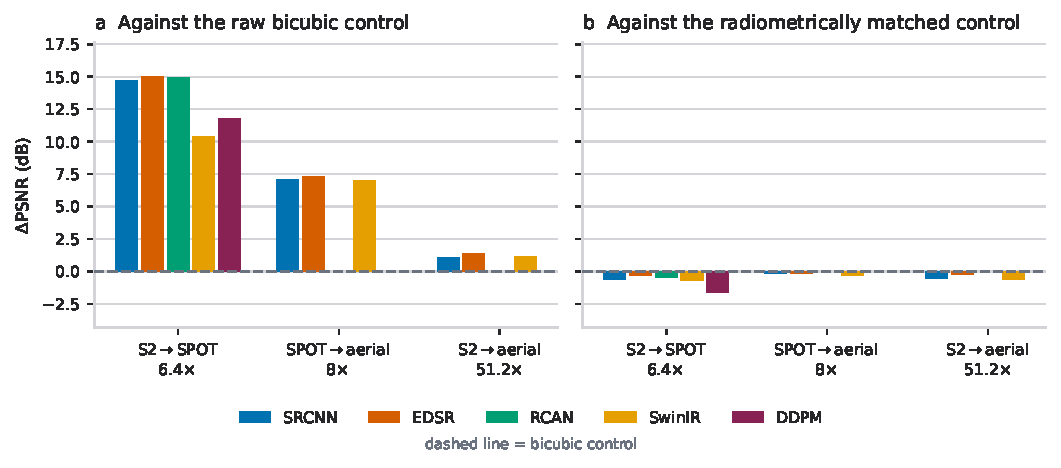
\includegraphics[width=\textwidth]{fig_psnr_paradox.pdf}
    \caption{The same SR models evaluated against two controls.
    \textbf{(a)} Against raw bicubic interpolation, apparent PSNR gains
    reach approximately $15$~dB. \textbf{(b)} After symmetric
    per-image radiometric matching, the advantage becomes close to
    zero. The contrast between the two evaluations exposes the strong
    contribution of cross-sensor radiometric differences.}
    \label{fig:paradox}
\end{figure*}

Importantly, the small matched-PSNR differences do not imply that the
models fail to reconstruct spatial information. As shown in
Fig.~\ref{fig:perceptual}, the SR outputs contain substantially more
high-frequency content than bicubic interpolation, and the amount
depends strongly on architecture. For SPOT$\rightarrow$aerial,
SwinIR reaches $5.55\times$ the bicubic sharpness (single seed),
followed by EDSR at $3.22\pm0.27\times$ and SRCNN at
$1.90\pm0.36\times$. For Sentinel-2$\rightarrow$aerial, the
corresponding single-seed ratios are $3.58\times$, $2.43\times$, and
$1.43\times$. In the smaller Sentinel-2$\rightarrow$SPOT gap, no
regression model exceeds the control: EDSR matches it
($1.00\times$), SwinIR falls slightly below ($0.91\times$), and RCAN
and SRCNN produce smoother outputs at $0.65\times$ and $0.59\times$.
These ratios are relative; in absolute terms, the bicubic control
retains only about $5\%$ of the target gradient magnitude $G(\mathbf{y})$ for
SPOT$\rightarrow$aerial, so even a $5.55\times$ ratio corresponds
to roughly a quarter of the target's gradient magnitude.

The diffusion model further illustrates the distinction between
perceptual quality and pixel fidelity. For
Sentinel-2$\rightarrow$SPOT, the conditional DDPM (single seed, one
sample per tile) reaches
$3.58\times$ the bicubic sharpness and an LPIPS of 0.2880 compared
with 0.5615 for the control, while its matched PSNR difference is
$-1.649$~dB. Thus, stronger high-frequency content and improved
perceptual similarity do not necessarily imply improved pixel-wise
fidelity, emphasizing the need to evaluate these properties jointly.

\begin{figure*}[!t]
    \centering
    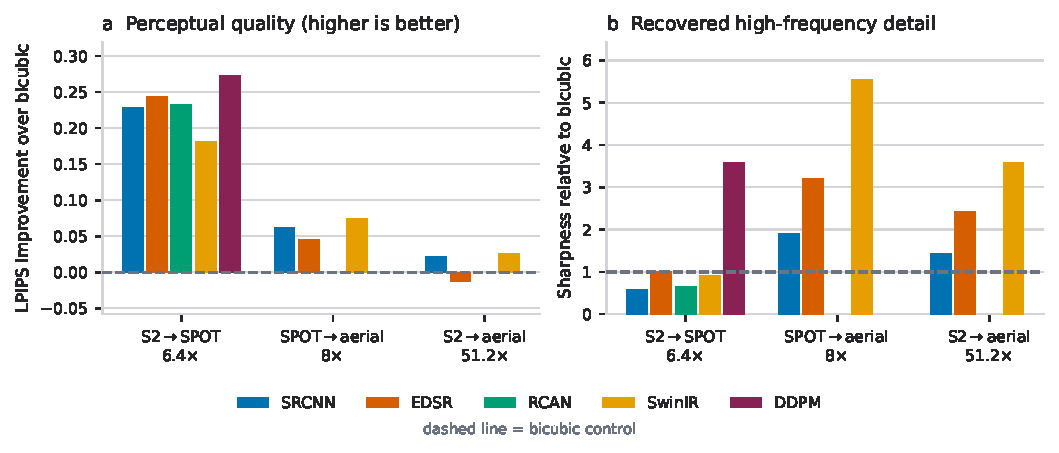
\includegraphics[width=\textwidth]{fig_perceptual.pdf}
    \caption{\textbf{(a)} LPIPS improvement relative to the bicubic
    control, $\mathrm{LPIPS}(\mathbf{x}_{\mathrm{bic}},\mathbf{y})-
    \mathrm{LPIPS}(\hat{\mathbf{y}},\mathbf{y})$ (higher is better).
    \textbf{(b)} Output sharpness $S$ relative to bicubic
    interpolation (Eq.~\ref{eq:bic_recovery}). The results show that models can recover substantial
    high-frequency content even when their radiometrically matched
    PSNR improvement is small or negative.}
    \label{fig:perceptual}
\end{figure*}

The land-cover analysis in Fig.~\ref{fig:perclass} further shows that
detail recovery depends on scene content. Class masks are the
FLAIR-HUB land-cover labels on the 0.20~m aerial grid. The analysis
uses SPOT$\rightarrow$aerial EDSR and EDSR+nDSM on 300 test tiles,
pooling every class pixel across tiles, and reports the eight most
frequent classes (each covering at least $0.5\%$ of pixels, i.e.,
more than $1.7$ million pixels per class). Because it uses one
trained model per variant, no per-class uncertainty is available, so
class-level differences of a few percentage points should be read as
indicative rather than statistically established. Across structured vegetated
and built classes, EDSR recovers approximately $13$--$22\%$ of the
target gradient magnitude, while the elevation-guided variant reaches
approximately $14$--$24\%$. Agricultural regions show a particularly
large relative improvement: bicubic interpolation recovers only
$3.3\%$ of the target gradient magnitude, compared with $15.3\%$
for EDSR.

The recovery fraction must nevertheless be interpreted together with
the target's own gradient magnitude. Water reaches approximately
$54\%$ recovery without elevation guidance and $81\%$ with guidance,
but its target gradient magnitude is only 0.0070, compared with
approximately 0.021--0.032 for more structured classes. Conversely,
deciduous vegetation has a target gradient magnitude of 0.0271 but
achieves only $13.1\%$ recovery with EDSR. A large normalized recovery
fraction therefore does not necessarily correspond to a large amount
of absolute spatial information.



The nDSM experiment is a focused case study restricted to the
SPOT$\rightarrow$aerial configuration and the SRCNN and EDSR backbones;
it is not generalized here to the other sensor pairs. Incorporating target-resolution
nDSM increases the matched PSNR difference of EDSR from
$-0.178\pm0.099$~dB to $+0.022\pm0.054$~dB, while its sharpness relative to bicubic
increases from $3.08\times$ to $3.75\times$. LPIPS simultaneously
improves from 0.8696 to 0.7822. SRCNN shows the same behavior:
matched PSNR improves from $-0.183\pm0.126$~dB to
$-0.041\pm0.073$~dB, sharpness increases from $1.91\times$ to
$2.50\times$, and LPIPS decreases from 0.8521 to 0.7968. The
baselines in Table~\ref{tab:ndsm} are the unguided runs paired with
the guided ones and therefore differ slightly from the independent
sweep in Table~\ref{tab:abs} (e.g., EDSR sharpness $3.08\times$
versus $3.22\times$), which is within the seed spread.


The spread of the matched-PSNR difference is comparable to the change
in its mean, so the positive mean of EDSR+nDSM should be interpreted
as approximate parity with the matched bicubic control rather than
statistically established superiority. The shift is nevertheless
accompanied by stronger spatial-detail recovery and better perceptual
similarity while requiring only 11,299 additional parameters,
approximately $1\%$ of the EDSR parameter count. Detail recovery
improves in seven of the eight evaluated land-cover classes; for
built and impervious regions it increases from approximately
$21.5\%$ to $24.0\%$. The effect is not uniform, however: the plowed
class decreases from approximately $15.5\%$ to $13.0\%$. Within the
tested SPOT$\rightarrow$aerial setting, nDSM guidance therefore
improves several metrics and most classes, but its benefit is
class- and scene-dependent.

Fig.~\ref{fig:qual_a} provides complementary
qualitative evidence. The bicubic reconstructions remain visibly
smooth, particularly in regions containing fine texture and narrow
spatial structures, whereas the learned SR outputs recover sharper
boundaries and additional local detail. The qualitative results are
therefore consistent with the quantitative sharpness analysis: the SR
models recover measurable spatial structure even when the improvement
over a radiometrically matched control is small.

Overall, the experiments demonstrate that no single metric adequately
describes real cross-sensor SR. Raw PSNR can be dominated by
radiometric adaptation, whereas matched PSNR alone can understate
measurable spatial-detail recovery. At the same time, increased
sharpness does not guarantee faithful reconstruction. Cross-sensor SR
should therefore be evaluated jointly through radiometrically matched
fidelity, spatial-detail recovery, perceptual similarity, and
scene-dependent analysis.

\begin{figure}
    \centering
    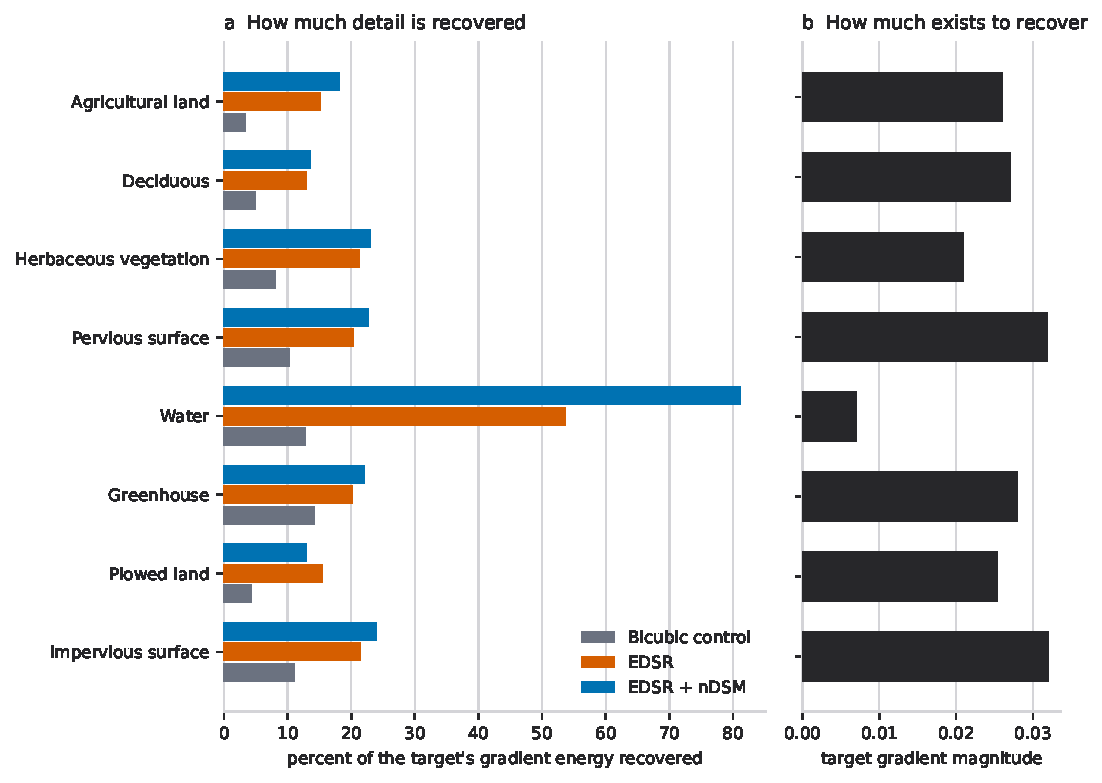
\includegraphics[width=\columnwidth]{fig_perclass.pdf}
    \caption{\textbf{(a)} Fraction of target spatial detail recovered
    by land-cover class. \textbf{(b)} Target gradient magnitude for
    each class. The target-gradient panel is required to interpret
    normalized recovery values across surfaces with different intrinsic
    spatial structure.}
    \label{fig:perclass}
\end{figure}

\begin{table}
\centering
\caption{Effect of Target-Resolution nDSM Guidance for
SPOT$\rightarrow$Aerial SR (Mean $\pm$ s.d.\ over Five Seeds; Paired
Baselines Trained Alongside the Guided Runs)}
\label{tab:ndsm}
\footnotesize
\setlength{\tabcolsep}{3.2pt}
\begin{tabular}{lccc}
\toprule
Method &
$\Delta_{\mathrm{matched}}$ (dB) &
Sharpness &
LPIPS $\downarrow$ \\
\midrule
SRCNN
& $-0.183\pm0.126$ & $1.91\times$ & 0.8521 \\
SRCNN+nDSM
& $-0.041\pm0.073$ & $2.50\times$ & 0.7968 \\
EDSR
& $-0.178\pm0.099$ & $3.08\times$ & 0.8696 \\
EDSR+nDSM
& $\mathbf{+0.022\pm0.054}$ &
  $\mathbf{3.75\times}$ &
  $\mathbf{0.7822}$ \\
\bottomrule
\end{tabular}
\end{table}

\begin{figure*}[!t]
    \centering
    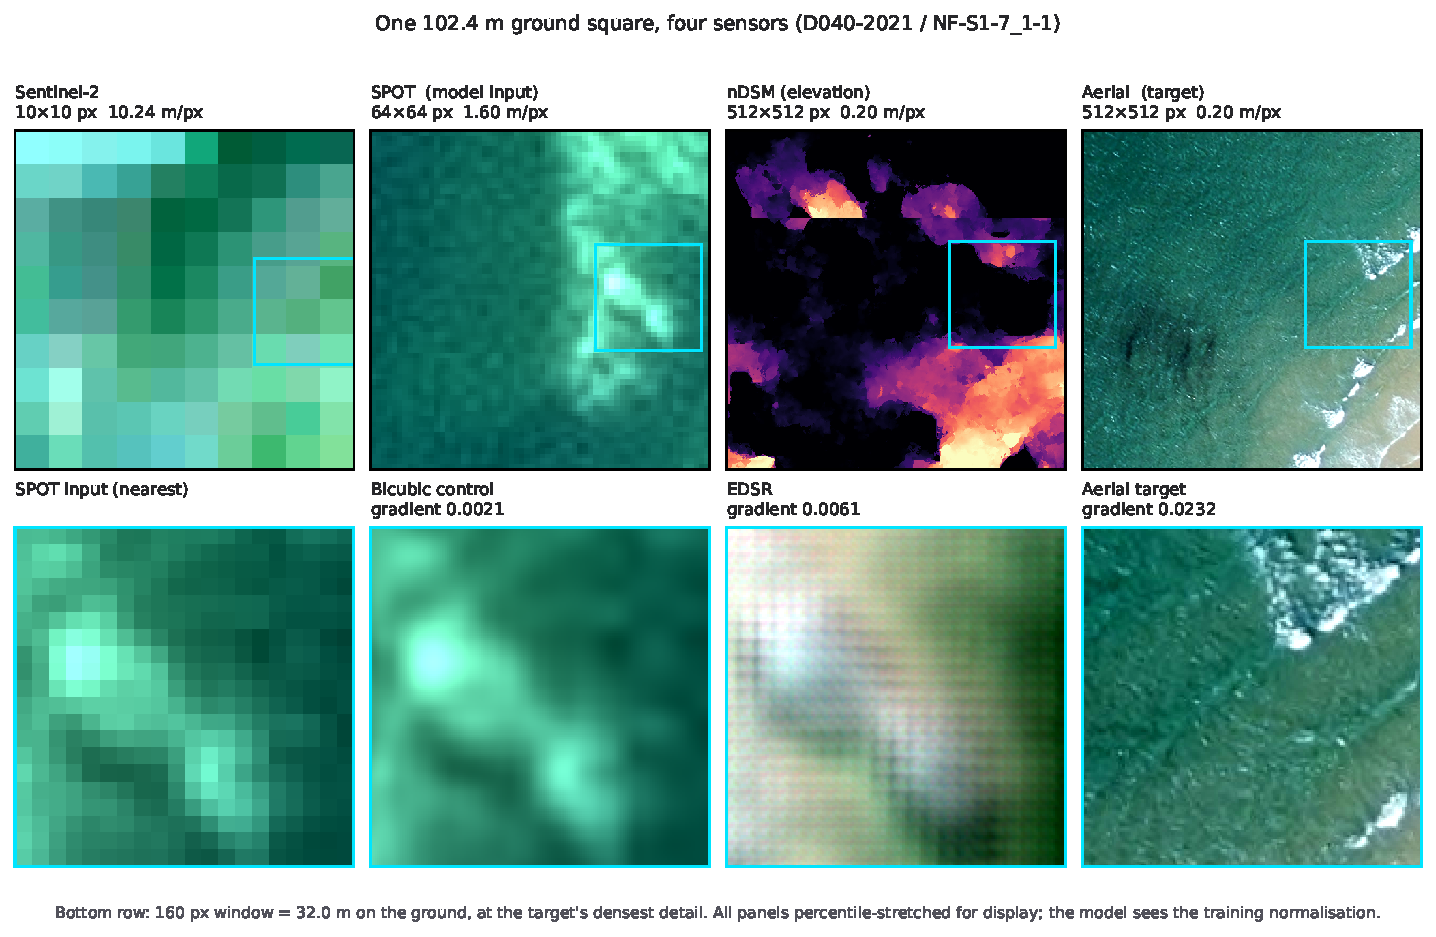
\includegraphics[width=0.8\textwidth]{fig_appendix_a.pdf}
    \caption{Representative qualitative cross-sensor SR results on
    held-out imagery. The comparison illustrates the progression from
    the low-resolution observation and bicubic control toward the SR
    reconstruction and high-resolution target.}
    \label{fig:qual_a}
\end{figure*}



\section{Conclusion}
\label{sec:conclusion}

This paper evaluated real cross-sensor satellite image
super-resolution using FLAIR-HUB across resolution gaps of
$6.4\times$--$51.2\times$. Results showed that apparent PSNR
gains approaching $15$~dB over raw bicubic interpolation
largely disappear after symmetric radiometric matching.
Nevertheless, SR models achieved up to $5.55\times$ higher
sharpness and recovered approximately $13$--$22\%$ of the
target gradient magnitude across structured land-cover classes.
In a focused SPOT$\rightarrow$aerial case study, nDSM guidance
brought EDSR to approximate matched-PSNR parity with the control
($-0.18$ to $+0.02$~dB), increased sharpness from $3.08\times$ to
$3.75\times$, and improved most, but not all, land-cover classes
with only $1\%$ additional parameters. These findings highlight
the importance of jointly evaluating radiometrically matched
fidelity, spatial-detail recovery, and perceptual quality
rather than relying on raw PSNR alone.

 
\bibliographystyle{IEEEtran}
\bibliography{refs}
 




% that's all folks
\end{document}


